\section{Preliminaries}\label{sec:ali_prelim}
We now review background relevant to our study. Our discussion focuses on knowledge graph representation models and aims to highlight the differences between \emph{shallow KG embedding} models such as the popular DistMult~\cite{distmult}, TransE~\cite{transe}, and ~RotatE~\cite{sun2019rotate} models and more recent \emph{reasoning-based embedding models}~\cite{ren2020query2box,ren2020beta}.
\subsection{Shallow Knowledge Graph Embeddings}\label{sec:ali_kg}
A knowledge graph (KG) $\gG=(\gV, \gE, \gR)$ consists of a set of nodes $\gV$, a set of edges $\gE$. $\gG$ also defines a set of relations $\gR$, and each edge $e\in\gE$ represents a triple $(v_s,r,v_o)$ where $r\in\gR$ and $v_s,v_o\in\gV$. Here, $v_s$ corresponds to the vector representation of the \texttt{subject} of the fact that corresponds to the edge and $v_o$ to the \texttt{object} of the fact. Finally, $r$ corresponds to the vector representation of the \texttt{predicate} associated with the triple.

Shallow KG embeddings~\cite{transe,distmult,sun2019rotate,trouillon2016complex} learn an embedding function $f_\theta$ that maps all the entities and relations on the graph to latent space in order to preserve the structure of graph. Most KG embeddings implement the embedding function $f_\theta$ as a matrix lookup. Specifically, the parameters include an entity embedding matrix $\rmV_\theta\in\R^{|\gV|\times d}$ and a relation embedding matrix $\rmR_\theta\in\R^{|\gR|\times d}$, where $d$ is the latent space dimension. 

\newparagraph{Training Shallow KG Embeddings:}
In order to train the two embedding matrices, these methods optimize a contrastive objective, which is to minimize a predefined distance function \texttt{Dist} of existing edges $e=(v_s,r,v_o)\in\gE$ while maximize that of non-existing edges $e'=(v_s,r,v_o')\notin\gE$. Different shallow KG embeddings have different definitions of the distance function \texttt{Dist}, the detail is listed in Table \ref{tab:kg-model}. 
In previous KG embedding works~\cite{sun2019rotate,zhang2019quaternion}, the loss function in the contrastive objective is defined as:
\begin{align} 
    \gL &= -\log \sigma \left(\gamma - \distt{v_s}{r}{v_o} \right) 
    - \sum_{j=1}^k \frac{1}{k} \log \sigma \left(\distt{v_s}{r}{v_{o_j}'} -\gamma \right),\label{eq:kgelossfunc}
\end{align}
where $\sigma$ is the sigmoid function, $\gamma$ is the margin. 
We optimize over the loss function using stochastic training for several iterations. In each iteration, these methods sample a batch of existing edges from the graph and construct non-existing edges by keeping the subject $v_s$ and the type of the edge $r$ fixed while perturbing the object $v_o$.


\begin{table}[t]
\small
\centering
\caption{The distance function of shallow KG embeddings and KG reasoning embeddings. 
\label{tab:kg-model}}
\resizebox{0.9\columnwidth}{!}{%
\begin{tabular}{ccc}
	\toprule
Model & Embedding Space & Distance \\
\hline
TransE~\cite{transe} & $\Em{v_s},\Em{v_o}\in\RR^d$, $\Em{r}\in\RR^d$ & $\|\Em{v_s}+\Em{r}-\Em{v_o}\|$ \\
\hline
RotatE~\cite{sun2019rotate} & $\Em{v_s},\Em{v_o}\in\CC^d$,$\Em{r}\in\CC^{d}$ & $\|\Em{v_s}\circ\Em{r}-\Em{v_o}\|$ \\\hline
DistMult~\cite{distmult} & $\Em{v_s},\Em{v_o}\in\RR^d$,$\Em{r}\in\RR^{d}$ & $-<\Em{v_s},\Em{r},\Em{v_o}>$ \\\hline
ComplEx~\cite{trouillon2016complex} & $\Em{v_s},\Em{v_o}\in\CC^{d}$, $\Em{r}\in\CC^{d}$ & $-\text{Re}(<\Em{v_s},\Em{r},\overline{\Em{v_o}}>)$ \\\hline
Q2B~\cite{ren2020query2box} & $\Em{v_s},\Em{v_o}\in\RR^{d}$, $\Em{r}\in\RR^{2d}$ & $\texttt{Dist}_\text{out}+\alpha\texttt{Dist}_\text{in}$ \\
% BetaE~\cite{ren2020beta} & $\Em{v_s},\Em{v_o}\in\RR^{d}$, $\Em{r}\in\RR^{d}$ & $\texttt{KL}(\text{Beta}(\Em{v_o});\text{Beta}(\texttt{MLP}(\Em{v_s},\Em{r})))$ \\

	\bottomrule
\end{tabular}
}%
\end{table}
\subsection{KG Reasoning Embeddings}\label{sec:ali_background}
KG reasoning embedding methods generalize the shallow KG embeddings to more complex reasoning tasks. KG reasoning embeddings also consider multi-hop reasoning over the KG, \ie, answering complex logical queries with logical/set operators including conjunction, disjunction and negation, \eg, \qu{Predict drugs that might target proteins that are associated with a given disease, and do not have a given side effect}~\cite{hamilton2018embedding}. 
In order to answer such complex queries, one may need to perform multiple reasoning steps and graph traversal -- first find all the proteins associated with the disease, and predict drugs $\gD_1 \subset \gV$ that bind with the proteins, at the same time find the drugs $\gD_2 \subset \gV$ that have the side effect and take complement of the set $\overline{\gD_2}$, and finally take the intersection of the two sets $\gD_1\cap\overline{\gD_2}$ to achieve the answers to the query. 
One of the main challenges of the above graph traversal method is that it suffers from missing and noisy information on the graph.
The key insight of KG reasoning embedding methods is to embed these complex queries in the same latent space as the entity embeddings so that all the reasoning steps can be done in the embedding space instead of symbolic graph traversal. 
In detail, we follow the logical queries defined in \citet{ren2020beta}. 
\begin{definition}[First-order logic queries]\label{def:query}
A first-order logic query $q$ consists of a non-variable anchor entity set $\gV_q \subseteq \gV$, existentially quantified bound variables $V_1, \dots, V_k$ and a single target variable $V_?$, which provides the query answer. The disjunctive normal form of a logical query $q$ is a disjunction of one or more conjunctions. 
\begin{align*}
\centering
    q[V_{?}] = V_?\:.\:\exists V_1, \ldots, V_k : c_1 \vee c_2 \vee ... \vee c_n
\end{align*}
\begin{enumerate}
    \item Each $c$ represents a conjunctive query with one or more literals $e$. $c_i = e_{i1} \wedge e_{i2} \wedge \dots \wedge e_{im}$.
    \item $e$ represents an atomic formula or its negation. $e_{ij} = r(v_a, V)$ or $\neg\:r(v_a, V)$ or $r(V', V)$ or $\neg\:r(V', V)$, where $v_a \in \gV_q$, $V \in \{V_?,V_1,\ldots,V_k\}$, $V' \in \{V_1,\ldots,V_k\}$, $V\neq V'$, $r \in \gR$.
\end{enumerate}
\end{definition}

% We can derive a computation graph for each query in Def.~\ref{def:query}. This computation graph represents the reasoning process in order to answer the query. Specifically, we can take each atomic formula $r(V_1, V_2)$ of the query and represent this formula with a graph with two nodes $V_1$ and $V_2$, and a directed edge $r$ that connects the two nodes. We merge the graphs of all atomic formula with logical edges including conjunction (set intersection), disjunction (set union) and negation (set complement). The merged graph will be the computation graph for this query. Each node of the computation graph represents a set of entities in the KG and each edge represents a logical/relational transformation of this set. 
% The computation graphs of FOL queries are heterogeneous \emph{trees}, where each leaf node corresponds to a set of cardinality one that contains a single anchor entity $v_a\in\gV_q$ (note that one anchor entity may appear in multiple leaf nodes) and the root node represents the unique target variable, which is the set of answer entities. 
% Each edge of the computation graph can take the following operations:
In order to reason over and embed such queries, one needs to consider the following operations. KG reasoning methods design neural logical operators that simulate their real counterparts. We refer the readers to \citep{ren2020query2box} for more details.
\begin{enumerate}
    \item \textbf{Relation Projection:} Given a set of entities $S \subseteq \gV$ and relation type $r \in \gR$, compute adjacent entities $\cup_{v \in S} A_r(v)$ related to $S$ via $r$: $A_r(v) \equiv \{v^{\prime} \in \gV: \ (v, r, v^{\prime})\in\gE\}$.
    \item \textbf{Intersection:} Given sets of entities $\{ S_1, S_2, \ldots, S_n\}$, compute their intersection $\cap_{i = 1}^n S_i$.
    \item \textbf{Complement/Negation:} Given a set of entities $S \subseteq \gV$, compute its complement $\overline{S} \equiv \gV \:\backslash\: S$.
    \item \textbf{Union:} Given sets of entities $\{ S_1, S_2, \ldots, S_n\}$, compute their union $\cup_{i = 1}^n S_i$.
\end{enumerate}


% To answer a given query, we can follow the query formula and execute logical operators. We denote the answer set as $\gA_q^\gG$, which represents the set of entities on $\gG$ that satisfy $q$, \textit{i.e.}, $v \in \gA_q^\gG \iff q[v]=\texttt{True}$. Note that this symbolic traversal of the computation graph is equivalent to traversing the KG, however, it has exponential computation complexity with respect to the number of hops and also cannot handle noisy or missing edges in the KG.

\newparagraph{Capturing Relational Context:} While KG reasoning queries have been traditionally proposed to answer complex queries in the presence of incomplete KGs, here, we utilize them to learn vector representations of the entities that are not biased towards one-hop relationships but take into account a richer \emph{relational context}. We use a set of \emph{query templates} (see Figure~\ref{fig:query}) to \emph{generate a sample workload of queries that can be answered over the input KG} and use that payload to learn robust entity representations as we discuss next. \emph{We experimentally show (see Section~\ref{sec:ali_experiment}) that this relational bias in the training process leads to entity representations that are more robust and lead to more stable representations (see Section~\ref{sec:ali_experiment}).}

\begin{figure}
        \centering
      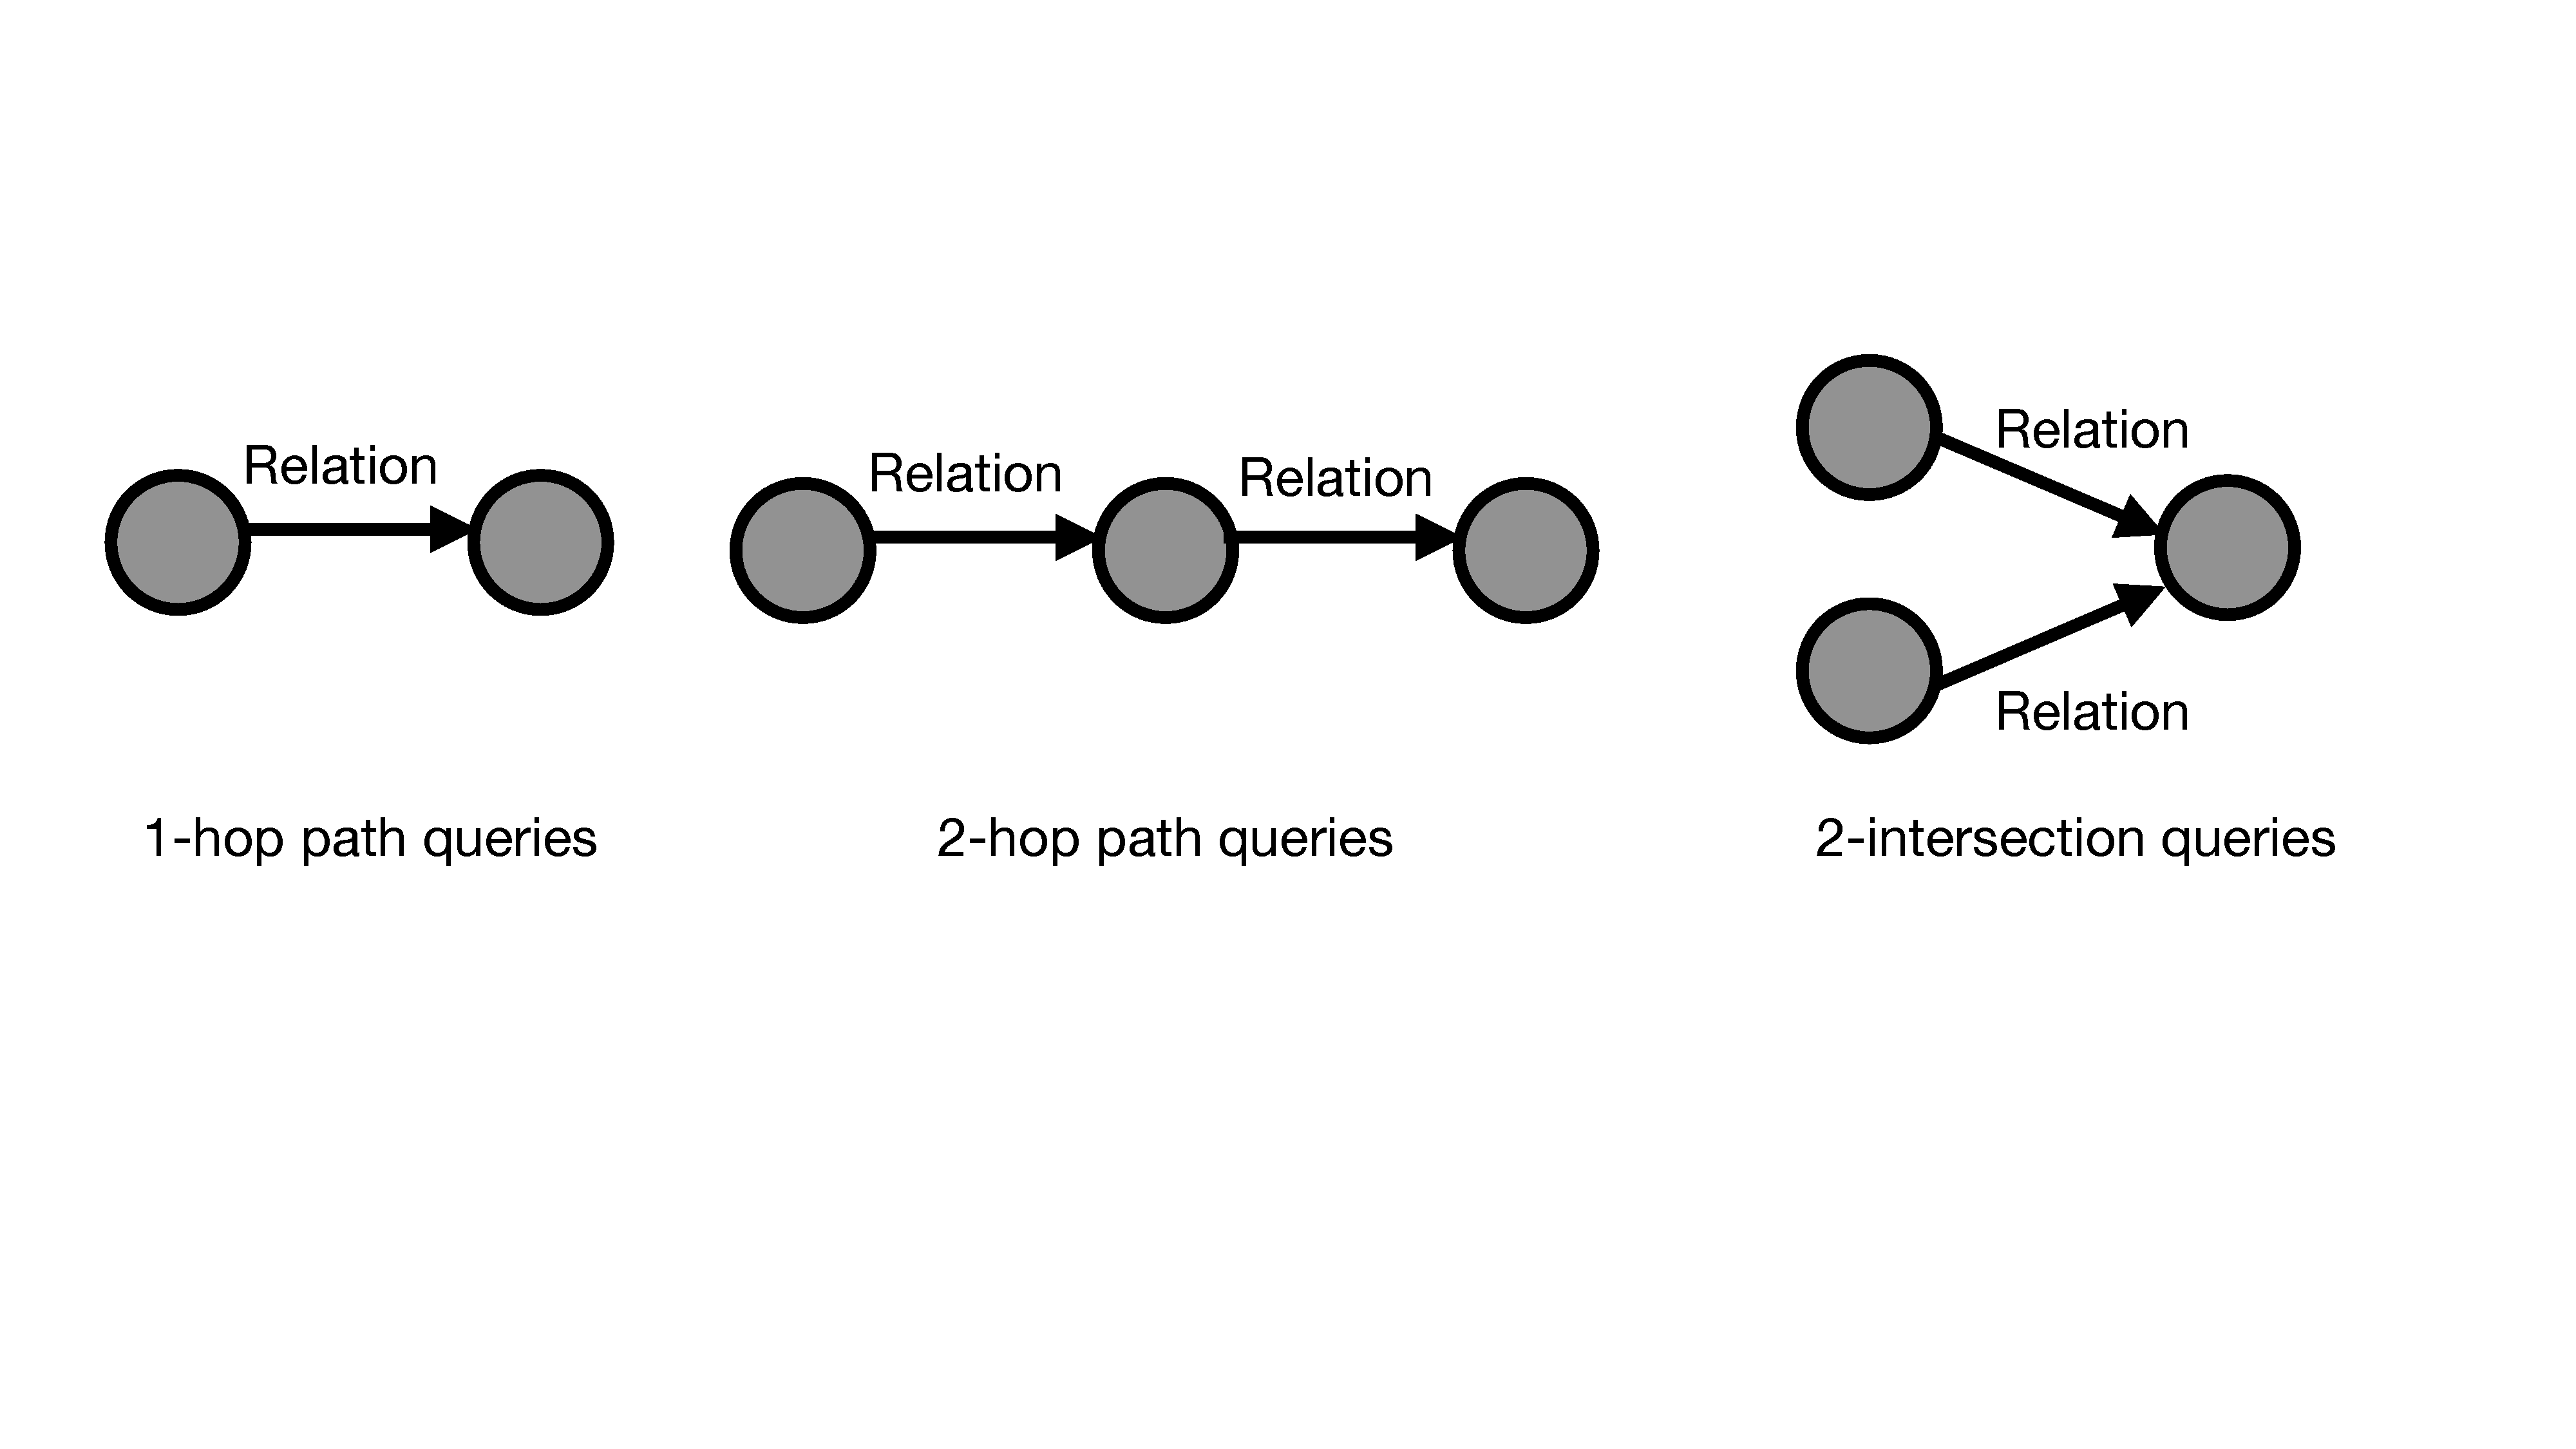
\includegraphics[width=0.5\columnwidth]{submissions/Ali2023/figures/query.pdf}
      \caption{Types of queries we consider to train Query2box.}
    \label{fig:query}
\end{figure}

\newparagraph{Training KG Reasoning Embeddings:} For a KG, $\gG = (\gV, \gE, \gR)$, and a query $q$, we need to learn an embedding function $f_\theta$ that maps from a computation graph of a query to its embedding with the parameterized neural logical operators. Together with the entity and relation embedding matrices (same as the shallow KG embeddings), $f_\theta$ also embeds all the nodes on the graph by embedding lookup. In order to measure the similarity/distance between a query $q$ and an entity $v \in \gV$, a distance function $\texttt{Dist}(\cdot,\cdot)$ is defined that takes as input the query embedding $f_\theta(q)$ and the entity embedding $f_\theta(v)$ and outputs the distance. The distance function $\texttt{Dist}(\cdot,\cdot)$ is tailored to different embedding space and model design $f_\theta$ as in Table \ref{tab:kg-model}.

During training, we are given a data sampler $\gD$, each sample in $\gD$ is a tuple $(q,\gA_q,\gN_q)$, which represents a query $q$, its answers $\gA_q\subseteq \gV$ and the negative samples $\gN_q\subseteq\overline{\gA_q}$. The training objective is to minimize the distance between the query embedding and its answers $\texttt{Dist}(q, v), v\in\gA_q$ while maximizing the distance between the query embedding and the negative samples $\texttt{Dist}(q, v'), v'\in\gN_q$, optimizing a contrastive loss term similar to the shallow KG embeddings. As used in most previous KG reasoning embedding works~\cite{ren2020beta,ren2020query2box}, the loss is defined as:
\begin{align} 
    \gL &= -\log \sigma \left(\gamma - \texttt{Dist}(q,v) \right) 
    - \sum_{j=1}^k \frac{1}{k} \log \sigma \left(\texttt{Dist}(q,v_j^{\prime})-\gamma \right),\label{eq:lossfunc}
\end{align}
where $\gamma$ is a margin hyperparameter and $\sigma$ is the sigmoid function. 
